\begin{center}
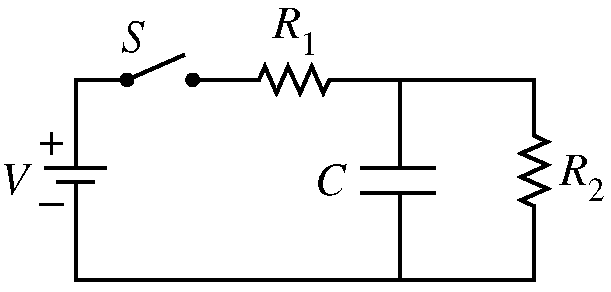
\includegraphics[scale=0.3]{images/img-009-010.png}
\end{center}

% Multiple Choice Question 17
\begin{questions}\setcounter{question}{16}\question
Capacitor $C$ and resistors $R_{1}$ and $R_{2}$ are connected to a battery as illustrated above. The capacitor is initially uncharged. The battery supplies constant voltage $V$ after the switch $S$ is closed at time $t=0$. Which of the following graphs best represents the current $I_{1}$ through the resistor $R_{1}$ as a function of $t$ ?

\begin{oneparchoices}
\choice \adjustbox{valign=t}{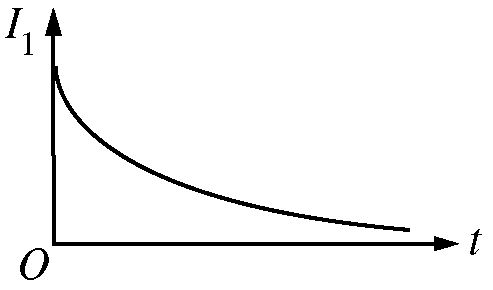
\includegraphics[scale=0.3]{images/img-009-011.png}}
\choice \adjustbox{valign=t}{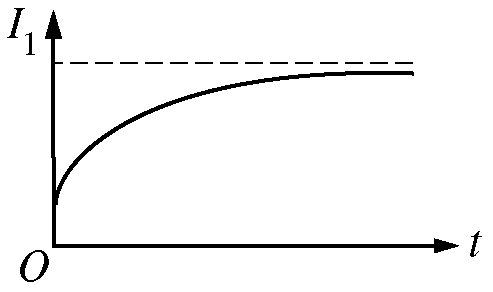
\includegraphics[scale=0.3]{images/img-009-012.png}}
\choice \adjustbox{valign=t}{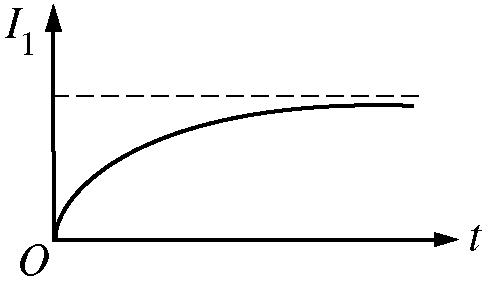
\includegraphics[scale=0.3]{images/img-009-013.png}}
\choice \adjustbox{valign=t}{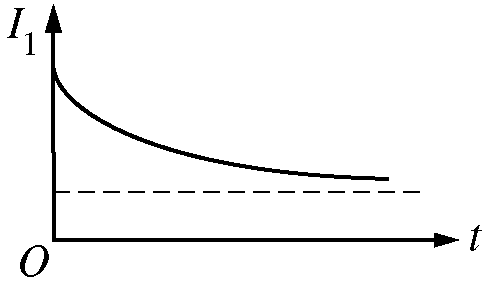
\includegraphics[scale=0.3]{images/img-009-014.png}}
\choice \adjustbox{valign=t}{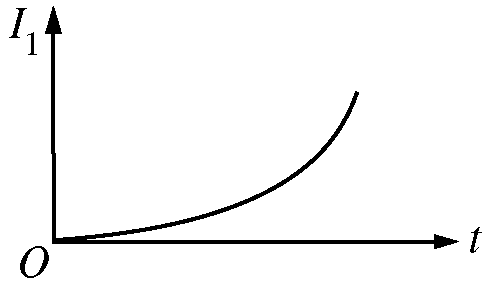
\includegraphics[scale=0.3]{images/img-009-015.png}}
\end{oneparchoices}\end{questions}

